\documentclass[10pt]{article}
\usepackage[margin=0.6in]{geometry}
\usepackage{tikz}
\usetikzlibrary{arrows.meta, positioning, fit, backgrounds, calc, shapes.geometric}
\usepackage{booktabs}
\usepackage{enumitem}
\usepackage{xcolor}
\usepackage{parskip}

\definecolor{ink}{HTML}{1A1A1A}
\definecolor{box}{HTML}{E8EEF7}
\definecolor{box2}{HTML}{F2E9DC}
\definecolor{box3}{HTML}{E4F1E8}
\definecolor{edge}{HTML}{555555}
\definecolor{warn}{HTML}{B03030}

\setlist[itemize]{leftmargin=3.5mm, itemsep=1pt, topsep=2pt, parsep=0pt}
\setlist[enumerate]{leftmargin=5mm, itemsep=1pt, topsep=2pt, parsep=0pt}

\newcommand{\qa}[2]{\item \textbf{#1} \, #2}
\newcommand{\code}[1]{\texttt{\small #1}}

\tikzset{
  n/.style={draw=edge, rounded corners=1.5pt, align=center, font=\scriptsize, inner sep=3pt, fill=white},
  nb/.style={n, fill=box},
  no/.style={n, fill=box2},
  ng/.style={n, fill=box3},
  db/.style={n, cylinder, shape border rotate=90, aspect=0.15, fill=box2},
  a/.style={-{Stealth[length=4pt]}, draw=edge, thin},
  ad/.style={a, dashed},
  lbl/.style={font=\tiny, midway, fill=white, inner sep=1pt},
  grp/.style={draw=gray!60, dashed, rounded corners, inner sep=3mm},
}

\pagestyle{plain}

\begin{document}

\begin{center}
{\LARGE\bfseries FocusLab --- Architecture Defense Sheet}\\[2pt]
{\small every branch someone can pull on, and the answer}
\end{center}

\vspace{-2mm}

\section*{0. Numbers}

\begin{tabular}{@{}p{3.2cm}p{4.4cm}p{9.4cm}@{}}
\toprule
\textbf{Claim} & \textbf{Value} & \textbf{Where it comes from} \\
\midrule
Services & 3 & \code{docker-compose.yml}: frontend :3000, backend :8000, agent :8001 \\
REST endpoints & 35 & canvas 1 + notebook 7 + queues 8 + keys 2 + spotify 12 + todo 5 \\
MCP tools & 11 & \code{FocusLab\_MCP/server.py}, 9 Canvas + 2 notes \\
Lines of code & $\approx$10{,}300 & py + ts + tsx across backend, agent, MCP, frontend/app \\
Models & 2 & Haiku 4.5 (chat agent), Sonnet 5 (page conversion) \\
Containers rebuilt & agent only & Tectonic + warm cache adds $\approx$110\,MB to that image \\
\bottomrule
\end{tabular}

\section*{1. System map}

\begin{center}
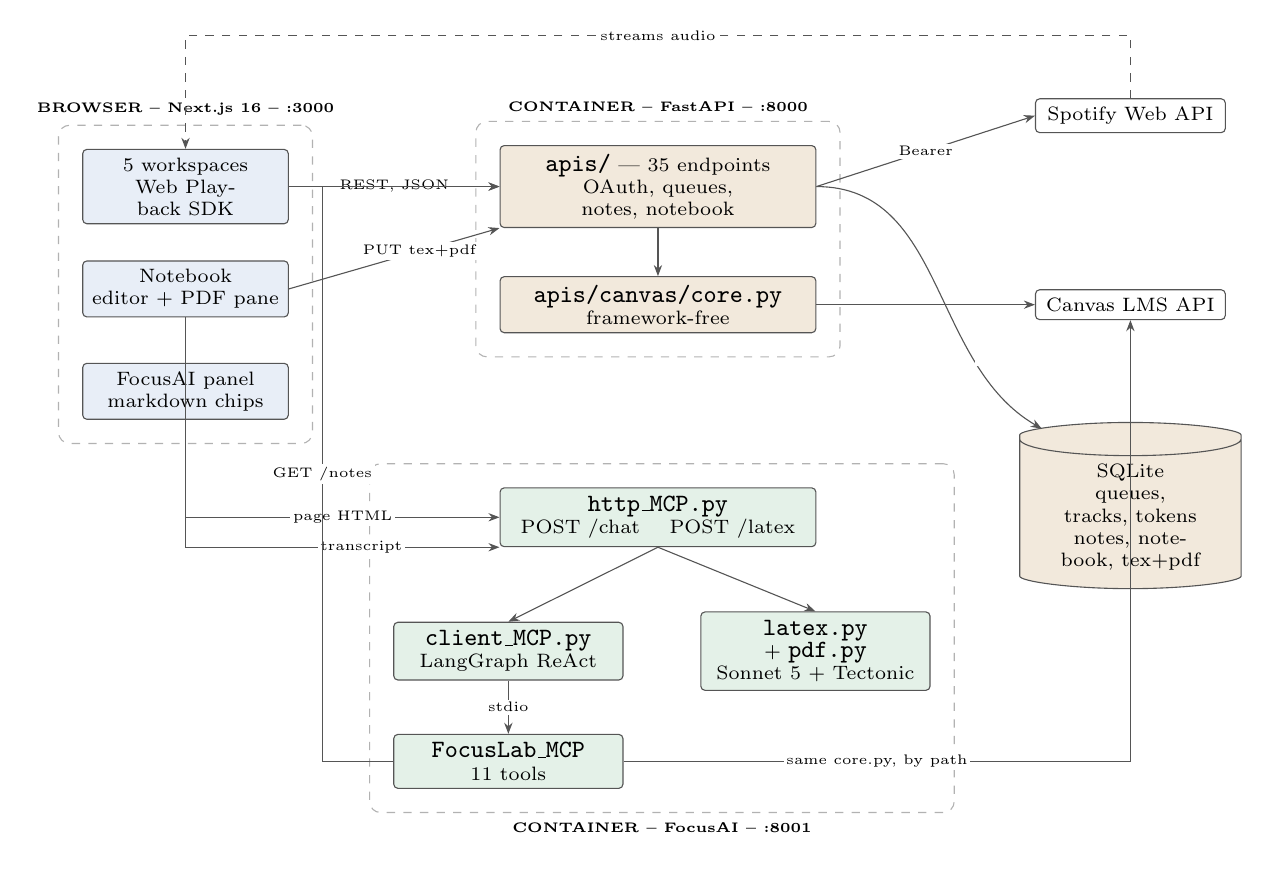
\begin{tikzpicture}[x=1cm, y=1cm]

% ---- browser column (x = 0) ----
\node[nb, text width=24mm] (ui)    at (0,  0.0) {5 workspaces\\Web Playback SDK};
\node[nb, text width=24mm] (note)  at (0, -1.3) {Notebook\\editor + PDF pane};
\node[nb, text width=24mm] (panel) at (0, -2.6) {FocusAI panel\\markdown chips};

% ---- backend column (x = 6) ----
\node[no, text width=38mm] (routes) at (6,  0.0) {\code{apis/} --- 35 endpoints\\OAuth, queues, notes, notebook};
\node[no, text width=38mm] (core)   at (6, -1.5) {\code{apis/canvas/core.py}\\framework-free};

% ---- agent column (x = 6, lower) ----
\node[ng, text width=38mm] (http) at (6, -4.2) {\code{http\_MCP.py}\\POST /chat \quad POST /latex};
\node[ng, text width=27mm] (loop) at (4.1, -5.9) {\code{client\_MCP.py}\\LangGraph ReAct};
\node[ng, text width=27mm] (tex)  at (8.0, -5.9) {\code{latex.py} + \code{pdf.py}\\Sonnet 5 + Tectonic};
\node[ng, text width=27mm] (mcp)  at (4.1, -7.3) {\code{FocusLab\_MCP}\\11 tools};

% ---- outside (x = 12) ----
\node[n,  text width=22mm] (spot)   at (12,  0.9) {Spotify Web API};
\node[n,  text width=22mm] (canvas) at (12, -1.5) {Canvas LMS API};
\node[db, text width=26mm] (dbn)    at (12, -4.2) {SQLite\\queues, tracks, tokens\\notes, notebook, tex+pdf};

% ---- edges ----
\draw[a] (ui.east)    -- node[lbl] {REST, JSON} (routes.west);
\draw[a] (note.east)  -- node[lbl, pos=0.62] {PUT tex+pdf} (routes.south west);
\draw[a] (note.south) |- node[lbl, pos=0.75] {page HTML} (http.west);
\draw[a] (panel.south) |- node[lbl, pos=0.78] {transcript} (http.south west);

\draw[a] (http.south) -- (loop.north);
\draw[a] (http.south) -- (tex.north);
\draw[a] (loop.south) -- node[lbl] {stdio} (mcp.north);

\draw[a] (routes.east) -- node[lbl] {Bearer} (spot.west);
\draw[a] (routes.south) -- (core.north);
\draw[a] (core.east)   -- (canvas.west);
\draw[a] (routes.east) to[out=0, in=150] node[lbl, pos=0.75] {} (dbn.north west);

\draw[a] (mcp.east) -| node[lbl, pos=0.25] {same core.py, by path} (canvas.south);
\draw[a] (mcp.west) -- ++(-0.9,0) |- node[lbl, pos=0.25] {GET /notes} (routes.west);
\draw[ad] (spot.north) -- ++(0,0.8) -| node[lbl, pos=0.25] {streams audio} (ui.north);

\begin{scope}[on background layer]
  \node[grp, fit=(ui)(note)(panel), label={[font=\tiny\bfseries]above:BROWSER -- Next.js 16 -- :3000}] {};
  \node[grp, fit=(routes)(core),    label={[font=\tiny\bfseries]above:CONTAINER -- FastAPI -- :8000}] {};
  \node[grp, fit=(http)(loop)(mcp)(tex), label={[font=\tiny\bfseries]below:CONTAINER -- FocusAI -- :8001}] {};
\end{scope}
\end{tikzpicture}
\end{center}

\textbf{Three facts this diagram is defending:} (1) the backend never touches audio --- the browser is the output device; (2) one Canvas implementation, two consumers; (3) the agent reaches user data through the REST API, not the database.

\newpage

\section*{2. Flow A --- FocusAI chat}

\begin{center}
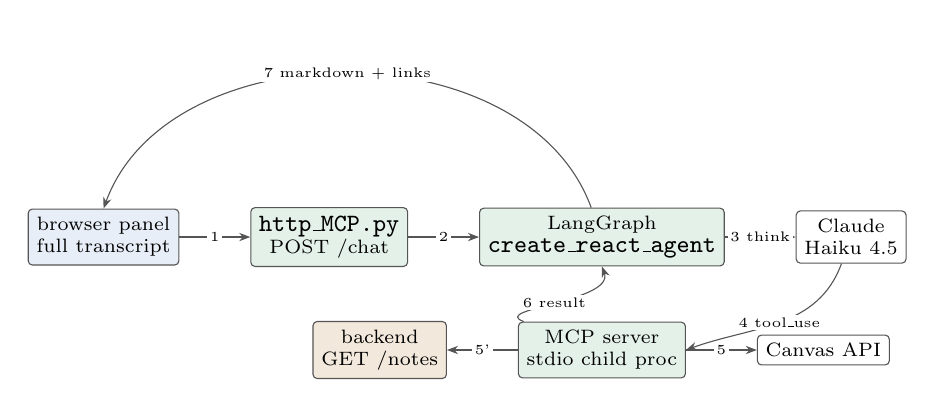
\begin{tikzpicture}[node distance=5mm]
\node[nb] (b) {browser panel\\full transcript};
\node[ng, right=9mm of b] (h) {\code{http\_MCP.py}\\POST /chat};
\node[ng, right=9mm of h] (g) {LangGraph\\\code{create\_react\_agent}};
\node[n, right=9mm of g] (m) {Claude\\Haiku 4.5};
\node[ng, below=7mm of g] (t) {MCP server\\stdio child proc};
\node[n, right=9mm of t] (c) {Canvas API};
\node[no, left=9mm of t] (r) {backend\\GET /notes};

\draw[a] (b) -- node[lbl] {1} (h);
\draw[a] (h) -- node[lbl] {2} (g);
\draw[a] (g) -- node[lbl] {3 think} (m);
\draw[a] (m) to[out=250, in=20] node[lbl] {4 tool\_use} (t.east);
\draw[a] (t) -- node[lbl] {5} (c);
\draw[a] (t) -- node[lbl] {5'} (r);
\draw[a] (t) to[out=160, in=290] node[lbl] {6 result} (g.south);
\draw[a] (g) to[out=110, in=70] node[lbl] {7 markdown + links} (b.north);
\end{tikzpicture}
\end{center}

\begin{itemize}
\qa{What is MCP?}{Open protocol: a server declares tools with JSON schemas, a client discovers and calls them. Transport here is \textbf{stdio} --- the agent spawns \code{server.py} as a child process.}
\qa{Why MCP over plain tool-calling?}{The tools are not welded to LangGraph. Same server works with any MCP client, and the REST API consumes the same Canvas core underneath.}
\qa{Why LangGraph?}{\code{create\_react\_agent} supplies the think$\to$call$\to$observe loop and message state. Model swap is one line.}
\qa{Why Haiku 4.5 here?}{Latency and cost per chat turn. Tool selection does not need frontier reasoning; the vision-heavy conversion uses Sonnet 5 instead.}
\qa{Where is the state?}{Nowhere. \code{/chat} is stateless: the browser owns the transcript and resends it whole. Two tabs never see each other's conversation.}
\qa{Why is the agent built once?}{\code{get\_tools()} spawns a Python process; rebuilding per message pays that startup every turn. Cached behind an \code{asyncio.Lock}.}
\qa{How do PDFs become clickable?}{Canvas file endpoints return \textbf{pre-signed} URLs. The agent emits them as markdown links; the panel renders markdown. Nothing is written to disk.}
\qa{Why not download server-side?}{\code{download\_files} writes to \code{\textasciitilde/Downloads} \emph{inside the container} --- not the user's machine. Links are the only thing that actually reaches them.}
\qa{The 11 tools}{\code{list\_courses, get\_modules, get\_assignments, get\_page\_files, get\_assignment\_files, download\_files, get\_grades, get\_assignment\_grades, get\_unsubmitted, list\_notes, read\_notes}}
\qa{Hallucination guards}{Prompt forbids inventing a course id --- every id must come from a tool result; \code{read\_notes} is illegal before \code{list\_notes}; course matching is substring, case-insensitive, over both \code{name} and \code{title}.}
\end{itemize}

\section*{3. Flow B --- Spotify auth + playback}

\begin{center}
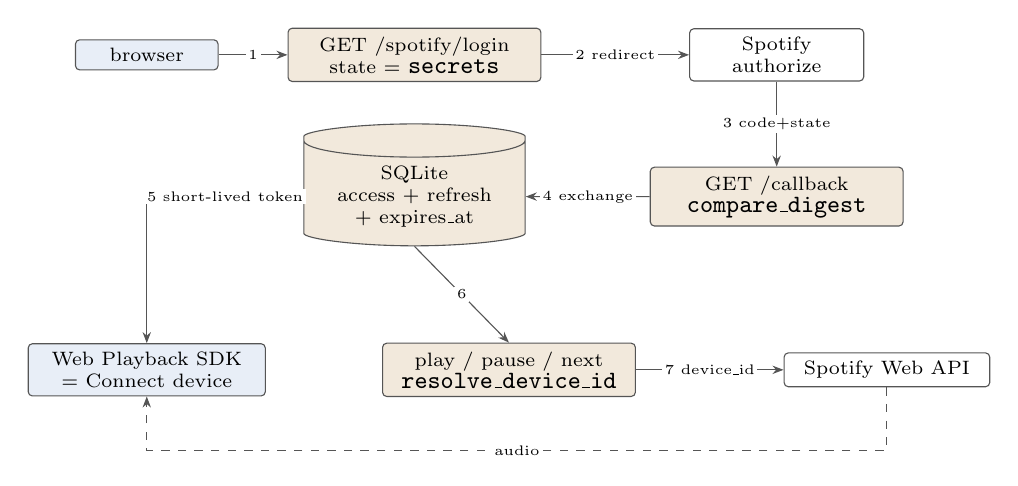
\begin{tikzpicture}[x=1cm, y=1cm]
\node[nb, text width=16mm] (b1)    at (0,    0.0) {browser};
\node[no, text width=30mm] (login) at (3.4,  0.0) {GET /spotify/login\\state = \code{secrets}};
\node[n,  text width=20mm] (sp)    at (8.0,  0.0) {Spotify\\authorize};
\node[no, text width=30mm] (cb)    at (8.0, -1.8) {GET /callback\\\code{compare\_digest}};
\node[db, text width=26mm] (tok)   at (3.4, -1.8) {SQLite\\access + refresh\\+ expires\_at};
\node[nb, text width=28mm] (sdk)   at (0,   -4.0) {Web Playback SDK\\= Connect device};
\node[no, text width=30mm] (cmd)   at (4.6, -4.0) {play / pause / next\\\code{resolve\_device\_id}};
\node[n,  text width=24mm] (api)   at (9.4, -4.0) {Spotify Web API};

\draw[a] (b1.east)    -- node[lbl] {1} (login.west);
\draw[a] (login.east) -- node[lbl] {2 redirect} (sp.west);
\draw[a] (sp.south)   -- node[lbl] {3 code+state} (cb.north);
\draw[a] (cb.west)    -- node[lbl] {4 exchange} (tok.east);
\draw[a] (tok.west)   -| node[lbl, pos=0.25] {5 short-lived token} (sdk.north);
\draw[a] (tok.south)  -- node[lbl] {6} (cmd.north);
\draw[a] (cmd.east)   -- node[lbl] {7 device\_id} (api.west);
\draw[ad] (api.south) -- ++(0,-0.8) -| node[lbl, pos=0.25] {audio} (sdk.south);
\end{tikzpicture}
\end{center}

\begin{itemize}
\qa{Which OAuth flow?}{Authorization Code. Client secret lives server-side, so no PKCE requirement --- the browser never sees a secret or a refresh token.}
\qa{Why server-side state, not a cookie?}{\code{\_pending\_login\_states} dict: 600\,s TTL, capped count, \textbf{single use}, matched with \code{secrets.compare\_digest} (constant-time). A replayed callback fails because the state was consumed.}
\qa{What stops CSRF exactly?}{An attacker cannot forge a state we handed out, and cannot reuse a real one --- one state, one callback.}
\qa{Where does refresh happen?}{Server-side, before every API call: \code{get\_valid\_access\_token} checks \code{expires\_at} and refreshes. The browser only ever gets a short-lived access token from \code{/spotify/token}.}
\qa{Why name the device explicitly?}{Spotify falls back to the \emph{active} device when a command names none. A freshly connected SDK player is \emph{visible but not active}, so an unnamed command plays nowhere. \code{resolve\_device\_id}: prefer \code{is\_active}, else first non-restricted, else 403 with a fix-it message.}
\qa{Error mapping}{401 $\to$ reconnect. 403 $\to$ pass Spotify's own wording (Premium / Extended Quota). ``Restriction violated'' $\to$ \textbf{409} (our polled state lagged, e.g. pausing an already-paused track). 404 $\to$ the device disappeared between resolve and command.}
\qa{Why \code{127.0.0.1} not \code{localhost}?}{Spotify banned \code{localhost} redirect URIs on 2025-11-27.}
\qa{Known constraint}{Playback control requires Premium; that is an account limit, not a bug.}
\end{itemize}



\section*{4. Flow C --- Notebook page $\to$ LaTeX $\to$ PDF}

\begin{center}
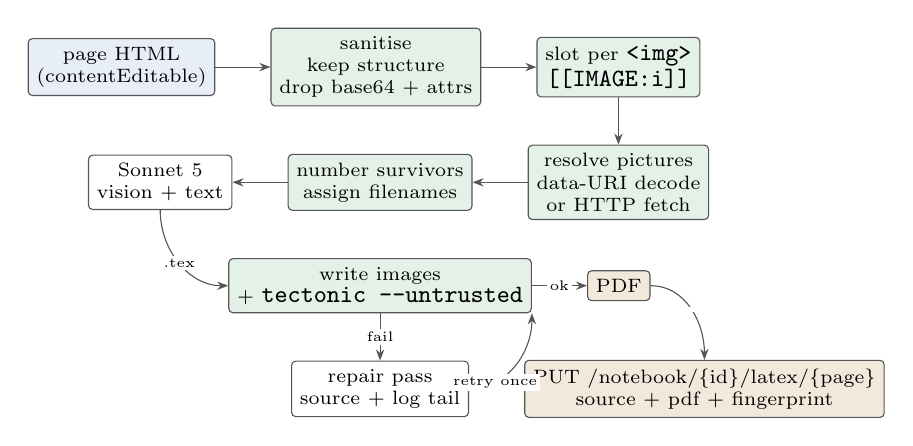
\begin{tikzpicture}[node distance=4mm]
\node[nb] (html) {page HTML\\(contentEditable)};
\node[ng, right=7mm of html] (san) {sanitise\\keep structure\\drop base64 + attrs};
\node[ng, right=7mm of san] (slot) {slot per \code{<img>}\\\code{[[IMAGE:i]]}};
\node[ng, below=6mm of slot] (fetch) {resolve pictures\\data-URI decode\\or HTTP fetch};
\node[ng, left=7mm of fetch] (num) {number survivors\\assign filenames};
\node[n, left=7mm of num] (claude) {Sonnet 5\\vision + text};
\node[ng, below=6mm of num] (tect) {write images\\+ \code{tectonic --untrusted}};
\node[no, right=7mm of tect] (ok) {PDF};
\node[n, below=6mm of tect] (rep) {repair pass\\source + log tail};
\node[no, right=7mm of rep] (store) {PUT /notebook/\{id\}/latex/\{page\}\\source + pdf + fingerprint};

\draw[a] (html) -- (san);
\draw[a] (san) -- (slot);
\draw[a] (slot) -- (fetch);
\draw[a] (fetch) -- (num);
\draw[a] (num) -- (claude);
\draw[a] (claude) to[out=270, in=180] node[lbl] {.tex} (tect.west);
\draw[a] (tect) -- node[lbl] {ok} (ok);
\draw[a] (tect) -- node[lbl] {fail} (rep);
\draw[a] (rep) to[out=0, in=270] node[lbl, pos=0.25] {retry once} (tect.south east);
\draw[a] (ok) to[out=0, in=90] node[lbl] {} (store.north);
\end{tikzpicture}
\end{center}

\begin{itemize}
\qa{Why sanitise instead of sending raw HTML?}{A pasted screenshot is megabytes of base64 --- it would blow the context and the model cannot read markup anyway. Structure is \emph{kept} (\code{h1--h4}, \code{b/i/u}, lists, inline colour) because that is exactly what maps to LaTeX commands.}
\qa{Why slots, then numbering?}{A linked picture may 404, be an SVG, or be too large. Numbers are only assigned to pictures actually in hand, so \code{\textbackslash includegraphics} can never name a file that was not written.}
\qa{Two kinds of image}{Pasted screenshot $\to$ \code{data:} URI, embedded. Pasted \emph{web page} $\to$ remote \code{https://} URL, fetched server-side (6 at a time, 12\,s timeout, type sniffed from magic bytes, not \code{Content-Type}).}
\qa{Transcribe or embed?}{Picture \emph{of text} (code, table, formula) $\to$ transcribed into \code{lstlisting} / \code{tabular} / math. Anything else, plus logos and badges $\to$ \code{\textbackslash includegraphics}. A code screenshot that stays a picture defeats the feature.}
\qa{Why Tectonic over TeX Live?}{One static binary + on-demand package bundle ($\approx$110\,MB total) against $\approx$2\,GB of apt. Build-time warm compile bakes the packages in, so the first real conversion does not wait on downloads.}
\qa{Security of compiling model output}{\code{--untrusted}: no shell-escape, no reads outside the working directory. Each compile runs in a temp dir deleted with everything in it.}
\qa{What if it will not compile?}{One repair pass --- the model gets its own source plus the log tail, told to fix only what the log names. Still failing $\to$ return the \textbf{original} transcription plus the log. The transcription is the valuable half; it is never lost to a compile error.}
\qa{Why Sonnet 5 and not Opus?}{Transcription + reading screenshots is a perception task, not a reasoning one. Verified on the hard case (code screenshot + diagram + typos + colour + escaping) --- Sonnet passed all of it.}
\qa{What does it correct?}{Spelling, punctuation, grammar, and plain-text math notation (\code{x\textasciicircum{}2} becomes $x^{2}$). Not: adding, removing, reordering, or restyling. It is a transcription contract, stated as an explicit may/may-not list in the prompt.}
\qa{Two prompt bugs found in testing}{(1) \code{\textbackslash maketitle} prints today's date unless \code{\textbackslash date\{\}} is set --- invented content. (2) Numbered \code{\textbackslash section} on a heading that already reads ``1 -- Pointers'' prints the number twice. Both fixed by rule, not by model choice.}
\qa{Why store the PDF, not recompile?}{A conversion costs an API call plus a compile. Re-opening a page must be free. Row keyed \code{(entry\_id, page\_index)}, unique.}
\qa{Staleness}{FNV-1a fingerprint of the page HTML is stored with it. On open, the live page is re-fingerprinted; mismatch $\to$ the pane says the page has changed. Never auto-deletes --- an out-of-date transcription still has value.}
\qa{Caps}{24 images/request (counted \emph{after} resolution), 60 candidates, 3.5\,MB per image, 20\,MB total, 120k HTML chars, 16k output tokens, 120\,s compile.}
\end{itemize}

\section*{5. Data model}

\begin{center}
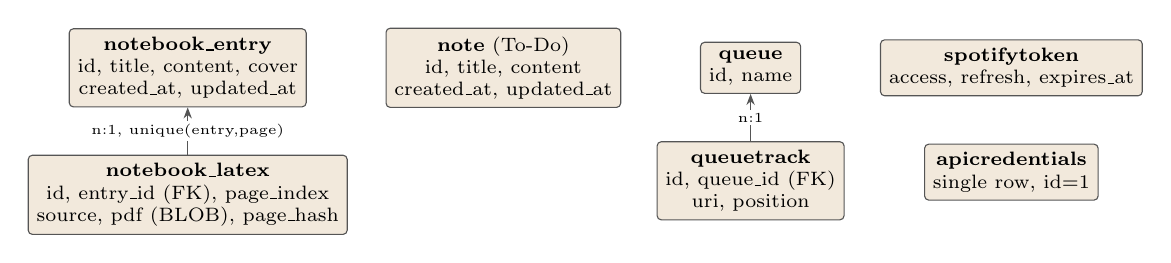
\begin{tikzpicture}[node distance=6mm]
\node[no] (ne) {\textbf{notebook\_entry}\\id, title, content, cover\\created\_at, updated\_at};
\node[no, below=6mm of ne] (nl) {\textbf{notebook\_latex}\\id, entry\_id (FK), page\_index\\source, pdf (BLOB), page\_hash};
\node[no, right=10mm of ne] (nt) {\textbf{note} (To-Do)\\id, title, content\\created\_at, updated\_at};
\node[no, right=10mm of nt] (q) {\textbf{queue}\\id, name};
\node[no, below=6mm of q] (qt) {\textbf{queuetrack}\\id, queue\_id (FK)\\uri, position};
\node[no, right=10mm of q] (st) {\textbf{spotifytoken}\\access, refresh, expires\_at};
\node[no, below=6mm of st] (ac) {\textbf{apicredentials}\\single row, id=1};

\draw[a] (nl) -- node[lbl] {n:1, unique(entry,page)} (ne);
\draw[a] (qt) -- node[lbl] {n:1} (q);
\end{tikzpicture}
\end{center}

\begin{itemize}
\qa{Why is there no \code{pages} table?}{An entry's pages live inside its own \code{content} HTML, split on a sentinel \code{<hr data-page-break>}. The MCP flattener and the To-Do renderer both survive that marker; a JSON array in \code{content} would have rendered as garbage in both.}
\qa{Why are Notebook and To-Do separate tables?}{They were one table, so an entry appeared on both pages and an edit on either moved the other. Split into \code{note} and \code{notebook\_entry}; neither model imports the other. The split \emph{copied} rather than moved --- which is what saved the data when a page was later blanked.}
\qa{Why SQLite?}{Single user, localhost, one file, zero ops. Nothing here needs concurrent writers.}
\qa{PDF in a BLOB --- really?}{$\approx$12--220\,KB per page, single user. The alternative (files on disk) adds a path to keep in sync with a row. Would not survive multi-user.}
\qa{Migration story}{\code{create\_all} builds new tables only. Column additions go through \code{\_ADDED\_COLUMNS}; the one-time note$\to$notebook copy is guarded by ``did \code{notebook\_entry} exist before \code{create\_all}'', which is true exactly once in a file's life.}
\end{itemize}



\section*{6. Decisions someone will push on}

\begin{tabular}{@{}p{4.1cm}p{5.6cm}p{7.3cm}@{}}
\toprule
\textbf{Chose} & \textbf{Over} & \textbf{Because} \\
\midrule
Agent in its own container & inside the FastAPI backend & LLM deps (langgraph, anthropic, Tectonic) and the Anthropic key stay out of the API image; backend has no use for either \\
Agent reads notes over REST & direct DB access & agent is a peer of the browser, not a privileged insider --- one door, one source of truth \\
\code{core.py} loaded by file path & pip-installable shared package & no packaging step, no web framework on the agent side; \code{importlib.util.spec\_from\_file\_location} \\
\code{/latex} in the agent container & in the backend & that is where the key and the engine are; it stores nothing, so the containers still share no database \\
Frontend stores the result & agent writes to the DB & keeps \code{/latex} stateless and keeps writes on the same path as every other save \\
Tectonic & TeX Live / a hosted service & 110\,MB vs 2\,GB; runs offline after the warm cache; no data leaves the machine \\
Sonnet 5 & Opus / Haiku & perception task, not reasoning; verified on the hardest page in the repo \\
uncontrolled contentEditable & React-controlled editor & a controlled rich-text surface fights the caret on every keystroke; imperative \code{innerHTML} + 600\,ms debounce instead \\
blob URL for the PDF & \code{data:} URL & browsers refuse to render \code{data:application/pdf} in a frame \\
\bottomrule
\end{tabular}

\section*{7. Failure modes and limits (say these before they find them)}

\begin{tabular}{@{}p{4.6cm}p{5.2cm}p{7.2cm}@{}}
\toprule
\textbf{Failure} & \textbf{What happens} & \textbf{Why that is the right behaviour} \\
\midrule
Agent container down & panel opens, says so & UI never fails silently \\
Document will not compile & source shown + engine log & the transcription is the valuable half \\
Linked image 404s / is SVG & \code{\% [image omitted]} & one dead logo must not fail a page \\
Image host is slow & 12\,s timeout, skipped & a page waiting on a CDN is worse than a missing picture \\
Page edited after converting & amber ``page has changed'' & stale $\ne$ wrong; user decides whether to re-spend \\
Spotify device vanishes & 404 mapped to a fix-it message & the state came from a poll and can lag \\
Two conversions at once & job counter drops the stale one & a late reply must not overwrite a newer pane \\
Editor not yet filled & saves are refused & see \S8 \\
\bottomrule
\end{tabular}

\section*{8. The bug worth telling}

\begin{itemize}
\item \textbf{Symptom.} A 37{,}513-character notebook entry went to 0 characters. Nobody deleted anything.
\item \textbf{Mechanism.} The editor is an uncontrolled \code{contentEditable} written by hand. Its sync effect returned early when the entry had not loaded yet, and its dependency list (\code{[activeNoteId, pageIndex]}) did not change when the entry \emph{arrived}. After a remount the div stayed empty while an entry was ``open''; the next save folded that empty div back into the entry.
\item \textbf{Detection.} A conversion test printed \code{page chars: 0}. The eslint \code{exhaustive-deps} warning had been pointing at this line the whole time.
\item \textbf{Recovery.} The pre-split copy still existed in the To-Do table, because the split copied rather than moved. Restored via \code{PATCH}, verified 26 images intact.
\item \textbf{Fix (two halves).} (1) The editor records which page it holds \emph{on the DOM node itself} (\code{dataset.page}) --- a freshly mounted div carries no marker, so a remount is always read as ``holds nothing'', with no state to reset. (2) No save path may fold in a div that is not marked for that page.
\item \textbf{Lesson to state out loud.} A lint warning that has been on screen for weeks is a bug that has not happened yet. And: a migration that copies instead of moves is a free backup.
\end{itemize}

\section*{9. Known gaps --- name them first}

\begin{itemize}
\item \textbf{No tests.} Verification is manual + scripted end-to-end runs against the live services. First thing to add: unit tests for the HTML sanitiser and the page-split helpers, which are pure functions.
\item \textbf{Remote image fetch is an SSRF surface.} The agent will fetch any \code{http(s)} URL found in a page's HTML, including private ranges. Single-user localhost limits the blast radius; a private-IP blocklist is the fix.
\item \textbf{No auth anywhere.} Both services trust the caller. CORS is an allowlist, and an allowlist is not authentication.
\item \textbf{SVG unsupported} in conversions --- neither the vision API nor the typesetter reads it. \code{cairosvg} + \code{libcairo2} would close it.
\item \textbf{Page indices shift.} Deleting page 2 makes the stored conversion for page 3 describe the wrong page; the fingerprint catches it as stale rather than silently mismatching.
\item \textbf{Stored PDFs grow the DB} unboundedly, one row per converted page.
\item \textbf{The agent only sees To-Do notes}, not Notebook entries --- deliberate after the split, since the two tables number from 1 independently and ids would collide.
\end{itemize}

\section*{10. Endpoint map}

\begin{tabular}{@{}p{2.4cm}p{1cm}p{13.6cm}@{}}
\toprule
\textbf{Prefix} & \textbf{n} & \textbf{Routes} \\
\midrule
\code{/spotify} & 12 & login, callback, status, token, player, devices, search, recently-played, next, previous, pause, resume \\
\code{/queues} & 8 & list, one, create, patch, delete, play, add track, delete track \\
\code{/notebook} & 7 & list, one, create, patch, delete, GET latex/\{page\}, PUT latex/\{page\} \\
\code{/notes} & 5 & list, one, create, patch, delete \\
\code{/keys} & 2 & status, save \\
\code{/canvas} & 1 & tasks \\
\midrule
agent :8001 & 2 & POST /chat, POST /latex \\
\bottomrule
\end{tabular}

\vspace{4mm}
\begin{center}
\footnotesize\itshape If you can draw \S1 on a whiteboard and tell the \S8 story, the rest is detail you can look up.
\end{center}

\end{document}
